\bf{Пример}

Пусть $N=6,$ $M=6,$ $Q=3,$ $X=[5,1,1,3,3,5],$ $Y=[1,2,3,4,0,2],$ $S=[4,4,5],$ $E=[2,2,4],$ $L=[1,2,3],$ и $R=[2,2,4].$

Проверяющий модуль \bf{(grader)} совершит вызов\t{ check_validity(6, [5, 1, 1, 3, 3, 5], [1, 2, 3, 4, 0, 2], [4, 4, 5], [2, 2, 4], [1, 2, 3], [2, 2, 4]).}

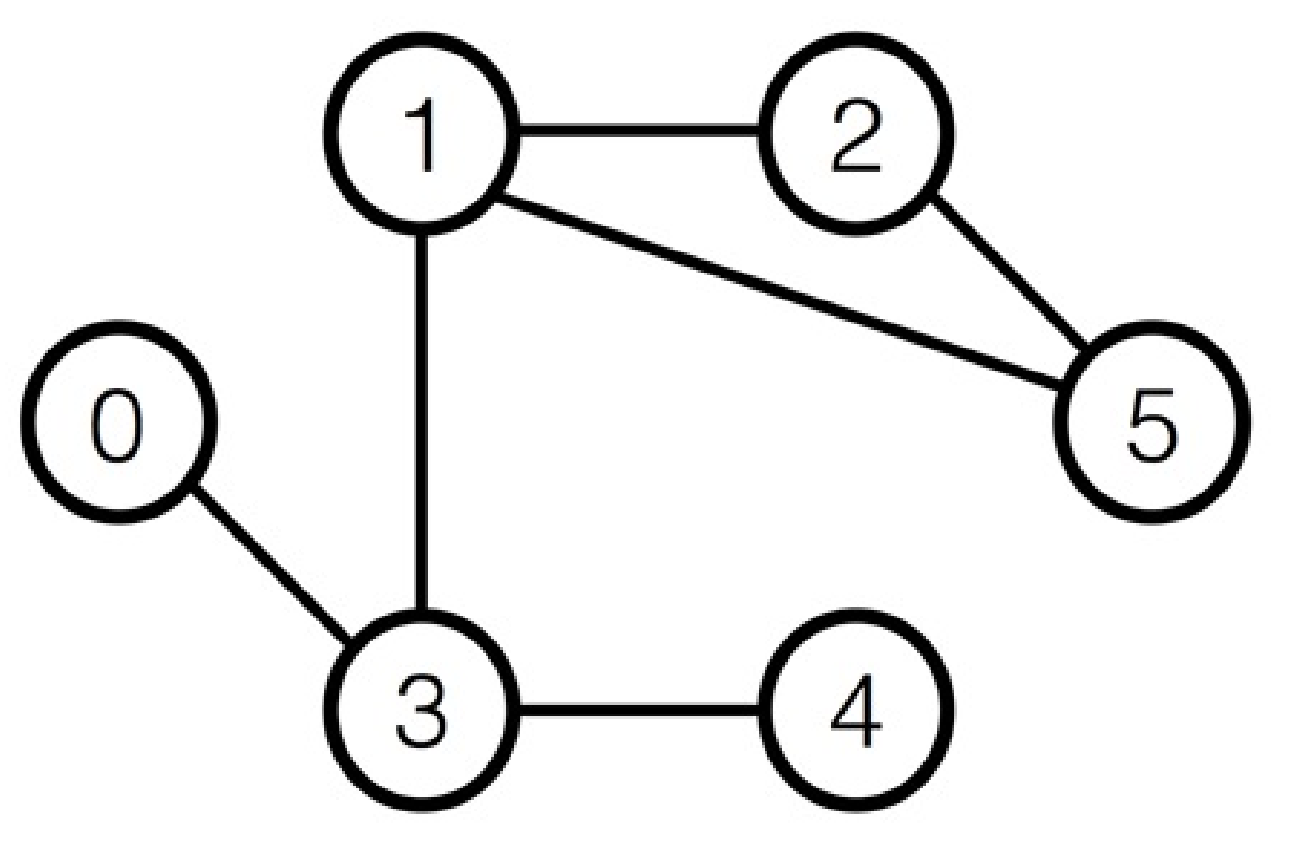
\includegraphics{image.png}

В путешествии $0$ можно добраться из города $4$ в город $2$ следующим образом:

\begin{itemize}
\item Начать в городе $4$ (Вы в форме человека) 
\item Переместиться в город $3$ (Вы в форме человека)
\item Переместиться в город $1$ (Вы в форме человека) 
\item Превратиться в волка (вы в форме волка) 
\item Переместиться в город $2$ (вы в форме волка)
\end{itemize}

В путешествиях $1$ и $2$ между данными парами городов переместиться невозможно.

Таким образом, ваша программа должна вернуть $[1,0,0].$

Файлы \t{sample-01-in.txt} и \t{sample-01-out.tx}t в приложенном архиве соответствуют этому примеру. В архиве также находятся другая пара файлов ввода и вывода, соответствующих еще одному примеру.

